%!TEX root = ../thesis.tex

\chapter{Implementation}
\label{ch:implementation}

\section{Introduction}

Text text

\subsection{Feature Overview}

To fully grasp what we need to implement, this section describes all the features we want to have QuickFeed support.

\textbf{Tasks and issues}

First of all we want QuickFeed to support teachers creating task markdown files within individual assignments.
As these are created and pushed to \textit{tests}, QuickFeed should create GitHub issues based on their contents in all group repositories.
Furthermore, when these task files are updated or deleted, their changes should be reflected in their respective issues.

\begin{figure}[ht]
    \centering
    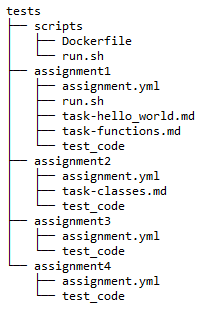
\includegraphics[scale=0.8]{photos/tests-repository-structure-tasks.PNG}
    \caption{Example of a tests repository with tasks}
    \label{fig:tests-repository-structure-tasks}
\end{figure}

\textbf{Pull Requests}

For every issue, group members are expected to solve them by creating a new branch and pull request.
QuickFeed should then support...
\begin{itemize}
    \item Returning automatic feedback every time a student pushes to a pull request.
    \item Automatically assigning appropriate reviewers when students get a passing score on their code.
    Specifically one teacher and one other group member.
    \item Correctly closing the pull request when a teacher approves it.
\end{itemize}

\section{Existing implementation}

An implementation has already been attempted for this project. % TODO: Ref here, and mention both names.
Before we can begin with a new one, we first have to decide which parts of it we want to use, and which to discard.
These parts are summarized in this section.

\subsection{SCM Expansion}
\label{sec:scm_expansion}

The SCM package has been expanded to support the following functions:

\begin{itemize}
    \item CreateIssue   - creates an issue on a repository.
    \item EditRepoIssue - edits an issue on a repository.
    \item GetRepoIssue  - retrieves an issue based on issue number and repository.
    \item GetRepoIssues - retrieves all issues from a repository.
\end{itemize}

CreateIssue and EditRepoIssue would prove useful, and are used with only minor adjustments to them.
The two other functions, centered around retrieving issues were not needed, but still used in earlier parts of the project when testing.

\subsection{Logic}

A lot of existing code was intended to handle the logic around managing tasks. 
In short, this code was meant to do determine when to create, edit or delete issues on GitHub.
The code did however not accomplish this in a functional manner.
This lead to the dilemma of whether to continue developing this faulty code, or simply start anew.
In the end, we decided that any attempt to fix the existing logic code would be more time consuming and confusing than simply starting fresh.

\subsection{Parsing Tasks}
\label{sec:parsing_tasks}

When a teacher pushes assignments to the \textit{tests} repository, QuickFeed will run the function UpdateFromTestsRepo.
In short, this function creates a local copy of the folder structure found in \textit{tests}, and uses it to create or update the data-record of every assignment.
Added as a part of this process, was code to also fetch all task markdown files in the repository, and use their contents to create a task data object.

To support this, all \textit{task-*.md} files are expected to conform to a standard format.
The first line should start with the character sequence "\# <task title>", followed by by two new line characters.
Any following text there after will be treated as the task body or description.

Using this format, the function newTask creates a task data object from any task file.

\lstinputlisting[caption={Function that creates a task object from markdown content}, language=Golang, firstline=25, lastline=40]{code/tasks.go}

Going forward, the general approach to parsing and creating tasks is left as it is, with only minor changes to the existing code.

\section{Managing Tasks and Issues}

Having looked at what existing code we decided to keep, we continue by exploring the part of the project that was implemented first; how to manage tasks and issues.

Moving forward in this chapter, we make the following distinction between found tasks/assignments, and existing tasks/assignments.
Found tasks and assignments are data objects created from the contents found within the \textit{tests} repository.
Existing tasks and assignments are data-objects based on data records that we retrieve from the database.

\subsection{Data Structures}

Two new messages are defined in the ag.proto file: \textbf{Task} and \textbf{Issue}.
These are used to generate the data structures that we use throughout the rest of the project.

\textbf{Task} is defined as follows:

\lstinputlisting[caption={Task message}, firstline=185, lastline=193]{code/ag.proto}

Every task is associated with one assignment via the \textit{assignmentID} field.

For an assignment, \textit{order} is a number used to determine the order in which it is represented in a course.
It is set by a teacher in the \textit{assignment.yml} file, which is described in section \ref{sec:quickfeed-repository-structure}.
When we create a new task, keeping track of the corresponding assignment order is useful.
It allows us to associate tasks and assignments without explicitly knowing the assignment ID, so long as our scope is limited to just a single course.
A feature that will prove necessary.

The \textit{name} field is used to associate tasks found in \textit{tests}, with the ones stored in the database.
If a task file with the name task-hello\_world.md is found within assignment1, then its corresponding name will be assignment1/hello\_world.
This name is set when the task itself is parsed, as described in section \ref{sec:parsing_tasks}.

\textbf{Issue} is defined as follows:

\lstinputlisting[caption={Issue message}, firstline=195, lastline=200]{code/ag.proto}

We see that every issue holds an association to the task that was used to create it, as well as the repository it was created on.

The \textit{issueNumber} field represents the issue number GitHub assigns the issue on its creation.

As it will become important in the next section, we will also mention that a modification was made to the existing message \textbf{Assignment}.

\lstinputlisting[caption={Assignment message}, firstline=168, lastline=183]{code/ag.proto}

On line 14 on the above code we see that the message has repeated tasks.
When we compile it, the resulting data structure can hold a list of tasks.

\subsection{Main Logic}

As mentioned in section \ref{sec:parsing_tasks}, UpdateFromTestsRepo is run when someone pushes to the \textit{tests} repository.
Since tasks and issues need to be synchronized every time this happens, all logic for doing so will happen here.

More specifically, we create the function handleTasks that manages all logic relating to tasks.
It is supplied with every found assignment, and their respective found tasks, as an argument.
The function itself is run at the end of UpdateFromTestsRepo.

\lstinputlisting[caption={The function handleTasks, responsible for all task related logic}, 
                language=Golang, label={code:handleTasks}, firstline=64, lastline=95]{code/tasks.go}

The logic contained in this function will be explained in the following sections.

\subsection{Synchronizing Tasks}

When teachers create, edit, and delete tasks, we must make sure that the same happens in QuickFeed's internal database.
To accomplish this, we create the database method SynchronizeAssignmentTasks.
This method is run at the start of handleTasks, and can be summarized in the following chart.

\begin{figure}[ht]
    \centering
    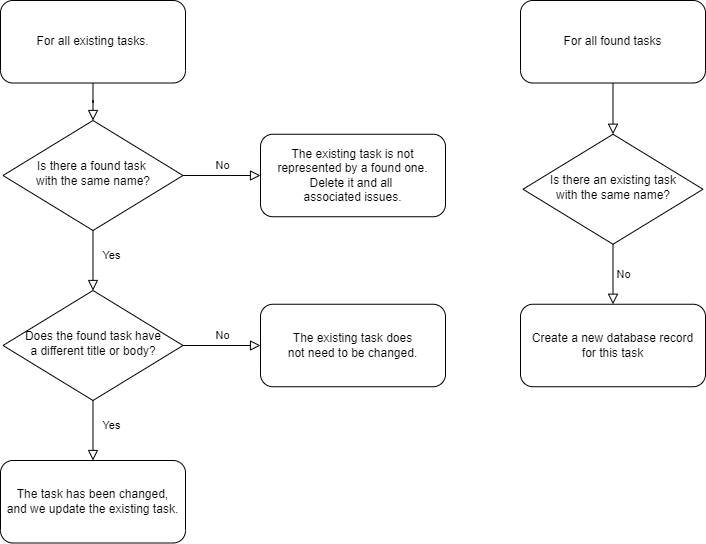
\includegraphics[width=\textwidth]{photos/synchronize-tasks-flow-chart.png}
    \caption{Flow chart describing how tasks are synchronized}
    \label{fig:synchronize-tasks-flow-chart}
\end{figure}

To support this logic, SynchronizeAssignmentTasks utilizes Go's built in maps to map tasks by both assignment order and name.
Given that we are limited in scope to a single course, we can use this mapping to associate every existing task to their found counterpart.

\lstinputlisting[caption={Logic performed in SynchronizeAssignmentTasks}, 
                language=Golang, label={code:SynchronizeAssignmentTasks}, firstline=41, lastline=76]{code/gormdb_tasks.go}

SynchronizeAssignmentTasks also returns the tasks it has created or updated, which will be important when synchronizing issues.

\subsection{Synchronizing Issues}

When we synchronize issues we must make sure to synchronize not only the issues stored in the database, but also the GitHub issues themselves.

As mentioned, SynchronizeAssignmentTasks already determines which tasks have been created, updated or deleted.
In fact, when it detects that a task has been deleted, it deletes not only the task but all associated issue records, as seen on line 11 in code \ref{code:SynchronizeAssignmentTasks}.
Issue data records also never need to be updated, since they carry no other information than an issue number, which always remains static.
The only remaining database related synchronization for issues is therefore creating them.

The entire process of synchronizing issues happens on line 16 to 31 in handleTasks \ref{code:handleTasks}.
In short, we use the created and updated tasks returned by SynchronizeAssignmentTasks, as arguments in createIssues and updateIssues respectively.
These functions use the SCM functions described in section \ref{sec:scm_expansion}.
Then, by looping through every course group repository we create and update GitHub issues accordingly.
createIssues also returns a list of all the issues it created.
These are used at the end of the process to create issue database records.

It is worth mentioning that there is no description on how we delete GitHub issues in the above process.
To delete issues, we wanted to expand on the SCM API to give it that capacity.
It turns out however, that GitHub's REST API does not support deleting issues.
An alternative could be to use GraphQL, a query language for API's, but instead we went for a simpler solution.
Instead of deleting issues, they are closed, and their title and body are inserted with a statement indicating that the associated task has been deleted.

\section{Managing Pull Requests}

Having implemented support for tasks and issues, we must now do the same for pull requests.

\subsection{Pull Request Data Structure}

To manage pull requests we need a data structure to represent them.
For this purpose, we create the \textbf{PullRequest} message.

\lstinputlisting[caption={PullRequest message}, firstline=202, lastline=217]{code/ag.proto} % TODO: Need to check for changes when finished

% TODO: Describe this message, and why certain fields are needed.

\subsection{Creating Pull Requests}

As students create pull requests to solve issues/tasks, we must make sure that a pull request record is created and stored internally to represent them.
Doing so allows us to keep track of which student is solving what task, who should be assigned to review the pull request, and more.
This section describes how this was implemented.

In section \ref{sec:creating-pull-requests} we decided on having students manually create pull requests.
To accommodate this feature, QuickFeed must react to the pull requests being opened.
Expanding QuickFeed to also handle pull request related webhooks, allows us to just that.

Specifically, when a pull request is opened we run the handlePullRequestOpened function.
It will check if a pull request is legitimate, i.e it was created on a group repository and linked to an appropriate issue.
If successful, the function creates a new record to represent it, by using the data in the event payload, and then stores it in the database.

Associating a pull request to an issue requires that the student themselves explicitly do so.
GitHub allows you to link issues to pull requests on their creation, by inserting a reference to them in the pull request body.
Doing so, we thought that the linked issue would also be part of the webhook payload.
This turned out to be incorrect, and instead we have to parse the issue number from the pull request body itself.

\subsection{Closing Pull Requests}

When students close and merge pull requests - ideally when they are supposed to - QuickFeed must also act accordingly.
Again, we use webhooks to listen to pull request closed events, and single out those that are relevant to QuickFeed.
By relevant we mean events for pull requests that already exist in QuickFeed's database, i.e they were created as part of the process described in the above section.
We can also filter out events for pull requests that were closed, but not merged.
This is because students need to merge the pull request into the main branch for QuickFeed to correctly score and grade the assignment as a whole.
Any non-merged pull request can therefore be ignored.

Assuming that the event is valid, we have two possible outcomes.
Either the pull request is approved, and we can safely delete it and its associated issue from the database.
Or, it has been closed and merged by a student without being explicitly approved by a teacher.
If this happens, QuickFeed must have the capacity to restore a working state for the issue/task in question.
To handle these situations, we only delete the pull request and not the issue record.
This way, a student doing an incorrect merge can simply reopen the issue that was closed, and then create a new pull request to represent it.
Thus restoring a working state with little QuickFeed involvement.

\section{Scoring Tasks}

To allow for both automatic and manual feedback, we need a way to score tasks.
Delivering automatic feedback requires us to do so solely on the tests associated with any given task.
Manual feedback on the other hand, needs some sort of task related score to determine when to assign reviewers.
Currently QuickFeed only tests and scores student code based on an assignment as a whole.
Having it do so on a per task basis therefore seems like a necessity to fulfill our goals.

QuickFeed's ci package is fundamentally designed to test assignments, therefore rewriting it to support tasks would be challenging.
Any solution might also not be backwards compatible.
To implement our features though, we do not explicitly need QuickFeed to test task related code, only score it.
As such, we can instead complement the score package to support this functionality.

Doing so turned out to be pretty straight forward.
First we changed the score message described in section \ref{sec:the-score-package} to also include a task name field.
By doing so, we have a direct reference to the task a given score is associated with.
Furthermore, to support teachers adding task specific tests, we created two new variants of the existing Add and AddSub methods.
Finally, to generate a total task specific score, we simply sum over the scores that have that task's name.

With these changes, we can generate a score from 0 - 100 for specific tasks, just as we already can for entire assignments.

\section{Manual Feedback}

\subsection{Assigning Reviewers}

\section{Automatic Feedback}

Not fully implemented yet.